\documentclass[a4paper, final]{article}
\usepackage{cmap}
%\usepackage{literat} % Нормальные шрифты
\usepackage[14pt]{extsizes} % для того чтобы задать нестандартный 14-ый размер шрифта
\usepackage[T2A]{fontenc}
\usepackage[UTF8]{inputenc}
\usepackage[russian]{babel}
\usepackage{listings} %листинги
\usepackage{amsmath}
\usepackage{amssymb} % Для красивого значка пустого множества
\usepackage[left=25mm, top=20mm, right=20mm, bottom=20mm, footskip=10mm]{geometry}
\usepackage{ragged2e} %для растягивания по ширине
\usepackage{setspace} %для межстрочного интервала
\usepackage{indentfirst} % для абзацного отступа
\usepackage{moreverb} %для печати в листинге исходного кода программ
\renewcommand\verbatimtabsize{4\relax}
\renewcommand\listingoffset{0.2em} %отступ от номеров строк в листинге
\renewcommand{\arraystretch}{1.4} % изменяю высоту строки в таблице
\usepackage[font=small, singlelinecheck=false, justification=centering, format=plain, labelsep=period]{caption} %для настройки заголовка таблицы
\usepackage{listingsutf8}
\usepackage{xcolor} % цвета
\usepackage{hyperref}% для гиперссылок
\usepackage{enumitem} %для перечислений
\usepackage{titlesec}
\usepackage{graphicx}
\graphicspath{ {./Рисунки/} }
%\usepackage{float}
\usepackage{booktabs}
\usepackage{floatrow}
\usepackage{scalerel} % Stretching images
\usepackage[final]{pdfpages}
\usepackage{multirow}
\usepackage{array}
\usepackage{tabularx}

\definecolor{apricot}{HTML}{FFF0DA}
\definecolor{mygreen}{rgb}{0,0.6,0}
\definecolor{string}{HTML}{B40000} % цвет строк в коде
\definecolor{comment}{HTML}{008000} % цвет комментариев в коде
\definecolor{keyword}{HTML}{1A00FF} % цвет ключевых слов в коде
\definecolor{morecomment}{HTML}{8000FF} % цвет include и других элементов в коде
\definecolor{captiontext}{HTML}{FFFFFF} % цвет текста заголовка в коде
\definecolor{captionbk}{HTML}{999999} % цвет фона заголовка в коде
\definecolor{bk}{HTML}{FFFFFF} % цвет фона в коде
\definecolor{frame}{HTML}{999999} % цвет рамки в коде
\definecolor{brackets}{HTML}{B40000} % цвет скобок в коде





\AtBeginDocument{\renewcommand{\contentsname}{Содержание}}
\AtBeginDocument{\renewcommand{\refname}{Список источников}}
% Настраиваем листинги, чтобы они использовали счётчик figure
\AtBeginDocument{
  \renewcommand{\thelstlisting}{\thefigure}  % Листинги используют тот же счетчик, что и рисунки
  \renewcommand{\lstlistingname}{Рис.}    % Меняем подпись
}

% Автоматически увеличиваем счетчик figure перед каждым листингом
\let\oldlstlisting\lstlisting
\renewcommand{\lstlisting}[1][]{%
    \refstepcounter{figure}% Увеличиваем счетчик figure
    \oldlstlisting[#1]% Вызываем оригинальную команду lstlisting
}
\lstset{
    captionpos=b
}
\newcommand{\specialcell}[2][l]{\begin{tabular}[#1]{@{}l@{}}#2\end{tabular}} % Алиас для таблиц

\floatsetup[table]{style=plain,capposition=top} % Подпись таблицы сверху
\setlist[enumerate,itemize]{leftmargin=1.2cm} %отступ в перечислениях

\hypersetup{colorlinks,
  allcolors=[RGB]{000 000 000}} %красивые гиперссылки (не красные)

% подгружаемые языки — подробнее в документации listings (это всё для листингов)
\lstloadlanguages{ [LaTeX] TeX}
% включаем кириллицу и добавляем кое−какие опции
\lstset{language =[LaTeX] TeX, % выбираем язык по умолчанию
extendedchars=true , % включаем не латиницу
escapechar = | , % |«выпадаем» в LATEX|
frame=tb , % рамка сверху и снизу
commentstyle=\itshape , % шрифт для комментариев
stringstyle =\bfseries} % шрифт для строк

\textheight=24cm % высота текста
\textwidth=16cm % ширина текста
\oddsidemargin=0pt % отступ от левого края
\topmargin=-1.5cm % отступ от верхнего края
\parindent=24pt % абзацный отступ
\parskip=0pt % интервал между абзацами
\tolerance=2000 % терпимость к "жидким" строкам
\flushbottom % выравнивание высоты страниц

\begin{document} % начало документа
\setcounter{tocdepth}{2} % Вложенность не больше 2 в содержании
\lstset{
  language=haskell, % Язык кода по умолчанию
  morekeywords={*,...}, % если хотите добавить ключевые слова, то добавляйте
  % Цвета
  keywordstyle=\color{keyword}\ttfamily\bfseries,
  %stringstyle=\color{string}\ttfamily,
  stringstyle=\ttfamily\color{red!50!brown},
  commentstyle=\color{comment}\ttfamily,
  morecomment=[l][\color{morecomment}]{\#},
  % Настройки отображения
  breaklines=true, % Перенос длинных строк
  basicstyle=\ttfamily\footnotesize, % Шрифт для отображения кода
  backgroundcolor=\color{bk}, % Цвет фона кода
  frame=single,xleftmargin=\fboxsep,xrightmargin=-\fboxsep, % Рамка, подогнанная к заголовку
  rulecolor=\color{frame}, % Цвет рамки
  tabsize=3, % Размер табуляции в пробелах
  % Настройка отображения номеров строк. Если не нужно, то удалите весь блок
  numbers=left, % Слева отображаются номера строк
  stepnumber=1, % Каждую строку нумеровать
  numbersep=5pt, % Отступ от кода
  numberstyle=\small\color{black}, % Стиль написания номеров строк
  % Для отображения русского языка
  extendedchars=true,
  literate={Ö}{ {\"O} }1
  {~}{ {\textasciitilde} }1
  {а}{ {\selectfont\char224} }1
  {б}{ {\selectfont\char225} }1
  {в}{ {\selectfont\char226} }1
  {г}{ {\selectfont\char227} }1
  {д}{ {\selectfont\char228} }1
  {е}{ {\selectfont\char229} }1
  {ё}{ {\"e} }1
  {ж}{ {\selectfont\char230} }1
  {з}{ {\selectfont\char231} }1
  {и}{ {\selectfont\char232} }1
  {й}{ {\selectfont\char233} }1
  {к}{ {\selectfont\char234} }1
  {л}{ {\selectfont\char235} }1
  {м}{ {\selectfont\char236} }1
  {н}{ {\selectfont\char237} }1
  {о}{ {\selectfont\char238} }1
  {п}{ {\selectfont\char239} }1
  {р}{ {\selectfont\char240} }1
  {с}{ {\selectfont\char241} }1
  {т}{ {\selectfont\char242} }1
  {у}{ {\selectfont\char243} }1
  {ф}{ {\selectfont\char244} }1
  {х}{ {\selectfont\char245} }1
  {ц}{ {\selectfont\char246} }1
  {ч}{ {\selectfont\char247} }1
  {ш}{ {\selectfont\char248} }1
  {щ}{ {\selectfont\char249} }1
  {ъ}{ {\selectfont\char250} }1
  {ы}{ {\selectfont\char251} }1
  {ь}{ {\selectfont\char252} }1
  {э}{ {\selectfont\char253} }1
  {ю}{ {\selectfont\char254} }1
  {я}{ {\selectfont\char255} }1
  {А}{ {\selectfont\char192} }1
  {Б}{ {\selectfont\char193} }1
  {В}{ {\selectfont\char194} }1
  {Г}{ {\selectfont\char195} }1
  {Д}{ {\selectfont\char196} }1
  {Е}{ {\selectfont\char197} }1
  {Ё}{ {\"E} }1
  {Ж}{ {\selectfont\char198} }1
  {З}{ {\selectfont\char199} }1
  {И}{ {\selectfont\char200} }1
  {Й}{ {\selectfont\char201} }1
  {К}{ {\selectfont\char202} }1
  {Л}{ {\selectfont\char203} }1
  {М}{ {\selectfont\char204} }1
  {Н}{ {\selectfont\char205} }1
  {О}{ {\selectfont\char206} }1
  {П}{ {\selectfont\char207} }1
  {Р}{ {\selectfont\char208} }1
  {С}{ {\selectfont\char209} }1
  {Т}{ {\selectfont\char210} }1
  {У}{ {\selectfont\char211} }1
  {Ф}{ {\selectfont\char212} }1
  {Х}{ {\selectfont\char213} }1
  {Ц}{ {\selectfont\char214} }1
  {Ч}{ {\selectfont\char215} }1
  {Ш}{ {\selectfont\char216} }1
  {Щ}{ {\selectfont\char217} }1
  {Ъ}{ {\selectfont\char218} }1
  {Ы}{ {\selectfont\char219} }1
  {Ь}{ {\selectfont\char220} }1
  {Э}{ {\selectfont\char221} }1
  {Ю}{ {\selectfont\char222} }1
  {Я}{ {\selectfont\char223} }1
  {\{}{ { {\color{brackets}\{} } }1 % Цвет скобок {
  {\} }{ { {\color{brackets}\} } } }1 % Цвет скобок }
}

% НАЧАЛО ТИТУЛЬНОГО ЛИСТА
\begin{center}
\hfill \break
\hfill \break
\normalsize{МИНИСТЕРСТВО НАУКИ И ВЫСШЕГО ОБРАЗОВАНИЯ РОССИЙСКОЙ ФЕДЕРАЦИИ\\
 федеральное государственное автономное образовательное учреждение высшего образования «Санкт-Петербургский политехнический университет Петра Великого»\\[5pt]}
\normalsize{Институт компьютерных наук и кибербезопасности}\\[5pt] 
\normalsize{Высшая школа технологий искусственного интеллекта}\\[5pt] 
\normalsize{Направление: 02.03.01 Математика и компьютерные науки}\\

\hfill \break
\hfill \break
\hfill \break
\large{\textbf{Технологии разработки ПО}}\\
\hfill \break
\large{<<Формальное описание процесса разработки модуля кодирования и декодирования графа кодом Прюфера с помощью методологии IDEF0>>}\\

\hfill \break
\hfill \break
\end{center}
 
\small{ 
\begin{tabular}{lrrl}
\!\!\!Студент, & \hspace{2cm} & & \\
\!\!\!группы 5130201/20102 & \hspace{2cm} & \underline{\hspace{3cm}} & Гаар В.С. \\\\
\!\!\!Преподаватель, \hspace{2cm} & & \\
\!\!\!к.т.н., доц. & \hspace{2cm} & \underline{\hspace{3cm}} &  Курочкин М.А. \\\\
&&\hspace{5cm}
\end{tabular}
\begin{flushright}
<<\underline{\hspace{1cm}}>>\underline{\hspace{2.5cm}} 2024 г.
\end{flushright}
}

\hfill \break
\hfill \break
\begin{center} \small{Санкт-Петербург, 2024} \end{center}
\thispagestyle{empty} % выключаем отображение номера для этой страницы

% КОНЕЦ ТИТУЛЬНОГО ЛИСТА
\newpage

\tableofcontents

\newpage

\cleardoublepage
\phantomsection
\addcontentsline{toc}{section}{Введение}
\section*{Введение}
Общая методология IDEF состоит из трех частных
методологий моделирования, основанных на графическом представлении
систем:
\begin{itemize}
  \item IDEF0 используется для создания функциональной модели, отображающей
  структуру и функции системы, а также потоки информации и материальных 
  объектов, связывающие эти функции.
  \item IDEF1 применяется для построения информационной модели, отображающей
  структуру и содержание информационных потоков, необходимых для 
  поддержки функций системы;
  \item IDEF2 позволяет построить динамическую модель меняющихся во времени
  поведения функций, информации и ресурсов системы.
\end{itemize}

В нашей работе используется методология IDEF0. Она позволяет исследовать функции организации, не связывая их с объектами, обеспечивающими их реализацию.

В данном случае объектом моделирования является процесс разработки модуля кодирования и декодирования графа 
кодом Прюфера.

\newpage
\section{Постановка задачи}
\noindent Для выполнения работы были поставлены следующие задачи:
\begin{enumerate}
	\item Изучить методологию IDEF0.
	\item В рамках этой методологии создать функциональную модель модуля кодирования и декодирования графа кодом Прюфера.
\end{enumerate}

\newpage
\section{Концепия IDEF0}
Методология IDEF0 основана на следующих концептуальных положениях.
\begin{enumerate}
	\item \textbf{Модель} --- искусственный объект, представляющий собой отображение (образ) системы и ее компонентов. Согласно \cite{bib:marka},

  \textbf{М} \textit{моделирует} \textbf{А}, \textit{если} \textbf{М} \textit{отвечает на вопросы относительно} \textbf{А}.

  Здесь \textbf{М} -- модель, \textbf{А} -- моделируемый объект (оригинал). Модель разрабатывают для понимания, анализа и принятия решений о реконструкции (реинжиниринге) или замене существующей, либо проектировании новой системы. Система представляет собой совокупность взаимосвязанных и взаимодействующих частей, выполняющих некоторую полезную работу. Частями  (элементами) системы могут быть любые комбинации разнообразных сущностей, включающие людей, информацию, программное обеспечение, оборудование, изделия, сырье или энергию (энергоносители). Модель описывает, что происходит в системе, как ею управляют, какие сущности она преобразует, какие средства использует для выполнения своих функций и что производит.

  \item \textbf{Блочное моделирование и его графическое представление.} Основной концептуальный принцип методологии IDEF --- представление любой изучаемой системы в виде набора взаимодействующих и взаимосвязанных блоков, отображающих процессы, операции, действия (определения -- см. ниже), происходящие в изучаемой системе. В IDEF0 все, что происходит в системе и ее элементах, принято называть \textbf{\textit{функциями}}. Каждой функции ставится в соответствие \textbf{\textit{блок}}. На \textbf{\textit{IDEF0-диаграмме}}, основном документе при анализе и проектировании систем, блок представляет собой прямоугольник. Интерфейсы, посредством которых блок взаимодействует с другими блоками или с внешней по отношению к моделируемой системе средой, представляются \textbf{\textit{стрелками}}, входящими в блок или выходящими из него. Входящие стрелки показывают, какие условия должны быть одновременно выполнены, чтобы функция, описываемая блоком, осуществилась.
  
  \item \textbf{Лаконичность и точность.} Документация, описывающая систему, должна быть точной и лаконичной. Многословные характеристики, изложенные в форме традиционных текстов, неудовлетворительны. Графический язык позволяет лаконично, однозначно и точно показать все элементы (блоки) системы и все отношения и связи между ними, выявить ошибочные, лишние или дублирующие связи и т.д..
  
  \item \textbf{Передача информации.} Средства IDEF0 облегчают передачу информации от одного участника разработки модели (отдельного разработчика или рабочей группы) к другому. К числу таких средств относятся:
  \begin{itemize}
    \item диаграммы, основанные на простой графике блоков и стрелок, легко читаемые и понимаемые;
    \item метки на естественном языке для описания блоков и стрелок, а также глоссарий и сопроводительный текст для уточнения смысла элементов диаграммы;
    \item последовательная декомпозиция диаграмм, строящаяся по иерархическому принципу, при котором на верхнем уровне отображаются основные функции, а затем происходит их детализация и уточнение;
    \item древовидные схемы иерархии диаграмм и блоков, обеспечивающие обозримость модели в целом и входящих в нее деталей.
  \end{itemize}

  \item \textbf{Строгость и формализм.} Разработка моделей IDEF0 требует соблюдения ряда строгих формальных правил, обеспечивающих преимущества методологии в отношении однозначности, точности и целостности сложных многоуровневых моделей. Эти правила описываются ниже. Здесь отмечается только основное из них: все стадии и этапы разработки и корректировки модели должны строго, формально документироваться с тем, чтобы при ее эксплуатации не возникало вопросов, связанных с неполнотой или некорректностью документации.
  
  \item \textbf{Итеративное моделирование.} Разработка модели в IDEF0 представляет собой пошаговую, итеративную процедуру. На каждом шаге итерации разработчик предлагает вариант модели, который подвергают обсуждению, рецензированию и последующему редактированию, после чего цикл повторяется. Такая организация работы способствует оптимальному использованию знаний системного аналитика, владеющего методологией и техникой IDEF0, и знаний специалистов -- экспертов в предметной области, к которой относится объект моделирования.
  
  \item \textbf{Отделение <<организации>> от <<функций>>.} При разработке моделей следует избегать изначальной «привязки» функций исследуемой системы к существующей организационной структуре моделируемого объекта (предприятия, фирмы). Это помогает избежать субъективной точки зрения, навязанной организацией и ее руководством. Организационная структура должна явиться результатом использования (применения) модели. Сравнение результата с существующей структурой позволяет, во-первых, оценить адекватность модели, а во-вторых -- предложить решения, направленные на совершенствование этой структуры. \cite{bib:gost_idef0}
\end{enumerate}

\newpage
\section{Основные понятия методологии и языка IDEF0}
\begin{enumerate}
  \item \textbf{\textit{Блок:}} прямоугольник, содержащий имя и номер и используемый для описания функции.
  \item \textbf{\textit{Ветвление:}} разделение стрелки на два или большее число сегментов.
  \item \textbf{\textit{Внутренняя стрелка:}} входная, управляющая или выходная стрелка, концы которой связывают источник и потребителя, являющиеся блоками одной диаграммы. Отличается от граничной стрелки.
  \item \textbf{\textit{Входная стрелка:}} класс стрелок, которые отображают вход IDEF0-блока, то есть данные или материальные объекты, которые преобразуются функцией в выход. Входные стрелки связываются с левой стороной блока IDEF0.
  \item \textbf{\textit{Выходная стрелка:}} класс стрелок, которые отображают выход IDEF0-блока, то есть данные или материальные объекты, произведенные функцией. Выходные стрелки связываются с правой стороной блока IDEF0.
  \item \textbf{\textit{Глоссарий:}} список определений для ключевых слов, фраз и аббревиатур, связанных с узлами, блоками, стрелками или с моделью IDEF0 в целом.
  \item \textbf{\textit{Граничная стрелка:}} стрелка, один из концов которой связан с источником или потребителем, а другой не присоединен ни к какому блоку на диаграмме. Отображает связь диаграммы с другими блоками системы и отличается от внутренней стрелки.
  \item \textbf{\textit{Декомпозиция:}} разделение моделируемой функции на функции-компоненты.
  \item \textbf{\textit{Дерево узлов:}} представление отношений между родительскими и дочерними узлами модели IDEF0 в форме древовидного графа.
  \item \textbf{\textit{Диаграмма A-0:}} специальный вид (контекстной) диаграммы IDEF0, состоящей из одного блока, описывающего функцию верхнего уровня, ее входы, выходы, управления, и механизмы, вместе с формулировками цели модели и точки зрения, с которой строится модель.
  \item \textbf{\textit{Диаграмма:}} часть модели, описывающая декомпозицию блока.
  \item \textbf{\textit{Диаграмма-иллюстрация (FEO):}} графическое описание, используе-
  мое, для сообщения специфических фактов о диаграмме IDEF0. При по-
  строении диаграмм FEO можно не придерживаться правила IDEF0.
  \item \textbf{\textit{Дочерний блок:}} блок на дочерней (порожденной) диаграмме.
  \item \textbf{\textit{Дочерняя диаграмма:}} диаграмма, детализирующая родительский (по-
  рождающий) блок.
  \item \textbf{\textit{Имя блока:}} глагол или глагольный оборот, помещенный внутри блока
  и описывающий моделируемую функцию.
  \item \textbf{\textit{Интерфейс:}} разделяющая граница, через которую проходят данные
  или материальные объекты; соединение между двумя или большим числом компонентов модели, передающее данные или материальные объекты от одного компонента к другому.
  \item \textbf{\textit{Код ICOM:}} аббревиатура (\textbf{I}nput -- Вход, \textbf{C}ontrol -- Управление, \textbf{O}utput -- Выход, \textbf{M}echanism -- Механизм), код, обеспечивающий соответствие граничных стрелок дочерней диаграммы со стрелками родительского блока; используется для ссылок.
  \item \textbf{\textit{Контекст:}} окружающая среда, в которой действует функция (или комплект функций на диаграмме).
  \item \textbf{\textit{Контекстная диаграмма:}} диаграмма, имеющая узловой номер A-n (\textbf{$n \geq 0$}), которая представляет контекст модели, Диаграмма A-0, состоящая из одного блока, является необходимой (обязательной) контекстной диаграммой; диаграммы с узловыми номерами A-1, A-2, ... -- дополнительные контекстные диаграммы.
  \item \textbf{\textit{Метка стрелки:}} существительное или оборот существительного, связанные со стрелкой или сегментом стрелки и определяющие их значение.
  \item \textbf{\textit{Модель IDEF0:}} графическое описание системы, разработанное с определенной целью и с выбранной точки зрения. Комплект одной или более диаграмм IDEF0, которые изображают функции системы с помощью графики, текста и глоссария.
  \item \textbf{\textit{Номер блока:}} число (0 - 6), помещаемое в правом нижнем углу блока и однозначно идентифицирующее блок на диаграмме.
  \item \textbf{\textit{Перечень узлов:}} список, часто ступенчатый, показывающий узлы модели IDEF0 в упорядоченном виде. Имеет то же значение и содержание, что и дерево узлов.
  \item \textbf{\textit{Примечание к модели:}} текстовый комментарий, являющийся частью диаграммы IDEF0 и используемый для записи факта, не нашедшего графического изображения.
  \item \textbf{\textit{Родительская диаграмма:}} диаграмма, которая содержит родительский блок.
  \item \textbf{\textit{Родительский блок:}} блок, который подробно описывается дочерней диаграммой.
  \item \textbf{\textit{Связывание/развязывание:}} объединение значений стрелок в составное значение (связывание в «пучок»), или разделение значений стрелок (развязывание <<пучка>>), выраженные синтаксисом слияния или ветвления стрелок.
  \item \textbf{\textit{Сегмент стрелки:}} сегмент линии, который начинается или заканчивается на стороне блока, в точке ветвления или слияния, или на границе (несвязанный конец стрелки).
  \item \textbf{\textit{Семантика:}} значение синтаксических компонентов языка.
  \item \textbf{\textit{Синтаксис:}} Структурные компоненты или характеристики языка и правила, которые определяют отношения между ними.
  \item \textbf{\textit{Слияние:}} объединение двух или большего числа сегментов стрелок в один сегмент. Может означать <<развязывание пучка>>
  лом компонентов модели, передающее данные или материальные объекты от одного компонента к другому.
  \item \textbf{\textit{С-номер:}} номер, создаваемый в хронологическом порядке и используемый для идентификации диаграммы и прослеживания ее истории; может быть использован в качестве ссылочного выражения при определении конкретной версии диаграммы.
  \item \textbf{\textit{Стрелка:}} направленная линия, состоящая из одного или нескольких сегментов, которая моделирует открытый канал или канал, передающий данные или материальные объекты от источника (начальная точка стрелки), к потребителю (конечная точка с «наконечником»). Имеется 4 класса стрелок: входная стрелка, выходная стрелка, управляющая стрелка, стрелка механизма (включает стрелку вызова). (См.: сегмент стрелки, граничная стрелка, внутренняя стрелка).
  \item \textbf{\textit{Стрелка вызова:}} вид стрелки механизма, который обозначает обращение из блока данной модели (или части модели) к блоку другой модели (или другой части той же модели) и обеспечивает связь между моделями или между разными частями одной модели.
  \item \textbf{\textit{Стрелка механизма:}} класс стрелок, которые отображают механизмы IDEF0, то есть средства, используемые для выполнения функции; включает специальный случай стрелки вызова. Стрелки механизмов связываются с нижней стороной блока IDEF0.
  \item \textbf{\textit{Стрелка, помещенная в туннель (туннельная стрелка):}} стрелка (со специальной нотацией), не удовлетворяющая обычному требованию, согласно которому каждая стрелка на дочерней диаграмме должна соответствовать стрелкам на родительской диаграмме.
  \item \textbf{\textit{Текст:}} любой текстовый (не графический) комментарий к графической диаграмме IDEF0.
  \item \textbf{\textit{Тильда:}} небольшая ломаная (волнистая) линия, используемая для соединения метки с конкретным сегментом стрелки или примечания модели с компонентом диаграммы.
  \item \textbf{\textit{Точка зрения:}} указание на должностное лицо или подразделение организации, с позиции которого разрабатывается модель
  \item \textbf{\textit{Узел:}} блок, порождающий дочерние блоки; родительский блок.
  \item \textbf{\textit{Узловая ссылка:}} код, присвоенный диаграмме, для ее идентификации и определения положения в иерархии модели; формируется из сокращенного имени модели и узлового номера диаграммы с дополнительными расширениями.
  \item \textbf{\textit{Узловой номер диаграммы:}} часть узловой ссылки диаграммы, которая соответствует номеру родительского блока.
  \item \textbf{\textit{Узловой номер:}} код, присвоенный блоку и определяющий его положение в иерархии модели; может быть использован в качестве подробного ссылочного выражения.
  \item \textbf{\textit{Управляющая стрелка:}} класс стрелок, которые в IDEF0 отображают управления, то есть условия, при выполнении которых выход блока будет правильным. Данные или объекты , моделируемые как управления, могут преобразовываться функцией, создающей соответствующий выход. Управляющие стрелки связываются с верхней стороной блока IDEF0.
  \item \textbf{\textit{Функция:}} деятельность, процесс или преобразование (моделируемые  блоком IDEF0), идентифицируемое глаголом или глагольной формой, которая описывает, что должно быть выполнено.
  \item \textbf{\textit{Цель:}} краткая формулировка причины создания модели. \cite{bib:gost_idef0}
\end{enumerate}

\newpage
\section{Синтаксис графического языка IDEF0}
Набор структурных компонентов языка, их характеристики и правила, определяющие связи между компонентами, представляют собой синтаксис языка.
Компоненты синтаксиса IDEF0-блоки, стрелки, диаграммы и правила. Блоки представляют функции, определяемые как деятельность, процесс, операция, действие или преобразование (см. ниже). Стрелки представляют данные или материальные объекты, связанные с функциями. Правила определяют, как следует применять компоненты; диаграммы обеспечивают формат графического и словесного описания моделей. Формат образует основу для управления конфигурацией модели.

\subsection{Блок}
Блок описывает функцию. Типичный блок показан на рис.~\ref{img:block}. Внутри каждого блока помещается его имя и номер. Имя должно быть активным
глаголом или глагольным оборотом, описывающим функцию. Номер блока размещается в правом нижнем углу. Номера блоков используются для их идентификации на диаграмме и в соответствующем тексте.

\begin{figure}[H]
   \centering
   
\includegraphics[width=0.7\linewidth]{block.png}
   \caption{Графическое представление блока}
   \label{img:block}
\end{figure}

\subsection{Стрелка}
Стрелка формируется из одного или более отрезков прямых и наконечника на одном конце. Как показано на рис.~\ref{img:arrows}, сегменты стрелок могут быть прямыми или ломаными; в последнем случае горизонтальные и вертикальные отрезки стрелки сопрягаются дугами, имеющими угол $90^\circ$. Стрелки не представляют поток или последовательность событий, как в традиционных блок-схемах потоков или процессов. Они лишь показывают, какие данные или материальные объекты должны поступить на вход функции для того, чтобы эта функция могла выполняться.

\subsection{Синтаксические правила}
\begin{figure}[H]
   \centering
   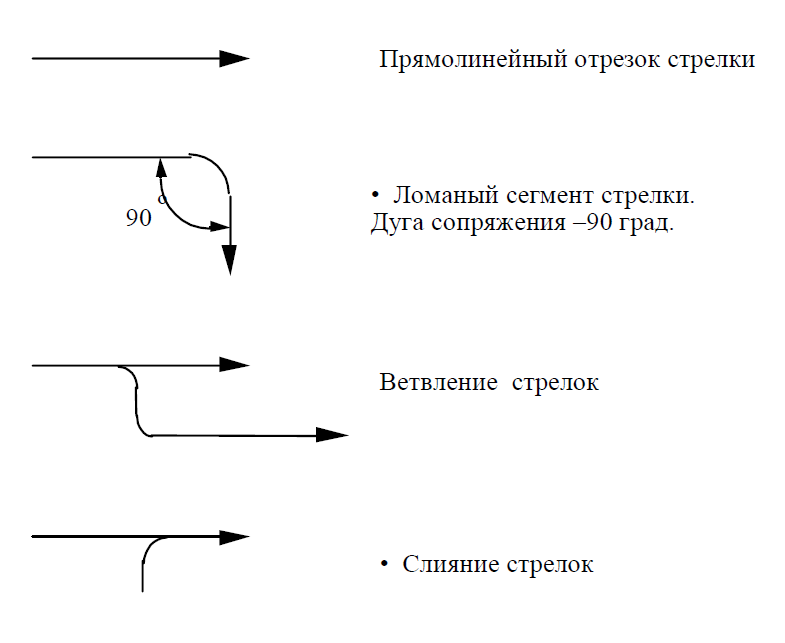
\includegraphics[width=0.7\linewidth]{arrows.png}
   \caption{Синтаксис стрелок}
   \label{img:arrows}
\end{figure}

\noindent \textbf{Блоки:}
\begin{enumerate}
  \item Размеры блоков должны быть достаточными для того, чтобы включить имя блока.
  \item Блоки должны быть прямоугольными, с прямыми углами.
  \item Блоки должны быть нарисованы сплошными линиями.
\end{enumerate}

\noindent \textbf{Стрелки:}
\begin{enumerate}
  \item Ломаные стрелки изменяют направление только под углом 90 град.
  \item Стрелки должны быть нарисованы сплошными линиями различной толщины.
  \item Стрелки могут состоять только из вертикальных или горизонтальных отрезков; отрезки, направленные по диагонали, не допускаются.
  \item Концы стрелок должны касаться внешней границы функционального блока, но не должны пересекать ее.
  \item Стрелки должны присоединяться к блоку на его сторонах. Присоединение в углах не допускается.
\end{enumerate}

\newpage
\section{Семантика языка IDEF0}
Семантика определяет содержание (значение) синтаксических компонентов языка и способствует правильности их интерпретации. Интерпретация устанавливает соответствие между блоками и стрелками с одной стороны и функциями и их интерфейсами -- с другой.

\subsection{Семантика блоков и стрелок}
Поскольку IDEF0 есть методология функционального моделирования, имя блока, описывающее функцию, должно быть глаголом или глагольным оборотом; например, имя блока "Выполнить проверку", означает, что блок с таким именем превращает непроверенные детали в проверенные. После присваивания блоку имени, к соответствующим его сторонам присоединяются входные, выходные и управляющие стрелки, а также стрелки механизма, что и определяет наглядность и выразительность изображения блока IDEF0. 

Чтобы гарантировать точность модели, следует использовать стандартную
терминологию. Блоки именуются глаголами или глагольными оборотами и эти имена сохраняются при декомпозиции Стрелки и их сегменты, как отдельные, так и связанные в «пучок», помечаются существительными или оборотами существительного. Метки сегментов позволяют конкретизировать данные или материальные объекты, передаваемые этими сегментами, с соблюдением синтаксиса ветвлений и слияний.

Каждая сторона функционального блока имеет стандартное значение с точки зрения связи блок/стрелки, В свою очередь, сторона блока, к которой присоединена стрелка, однозначно определяет ее роль. Стрелки, входящие в левую сторону блока -- входы. Входы преобразуются или расходуются функцией, чтобы создать то, что появится на ее выходе. Стрелки, входящие в блок сверху -- управления. Управления определяют условия, необходимые функции, чтобы произвести правильный выход. Стрелки, покидающие блок справа –- выходы, т.е. данные или материальные объекты, произведенные функцией. Стрелки, подключенные к нижней стороне блока, представляют механизмы. Стрелки, направленные вверх, идентифицируют средства, поддерживающие выполнение функции. Другие средства могут наследоваться из родительского блока. Стрелки механизма, направленные вниз, являются стрелками вызова. Стрелки вызова обозначают обращение из данной модели или из данной части модели к блоку, входящему в состав другой модели или другой части модели, обеспечивая их связь, т.е. разные модели или разные части одной и той же модели могут совместно использовать один и тот же элемент (блок). Стандартное расположение стрелок показано на рис.~\ref{img:semantics}.

\begin{figure}[H]
   \centering
   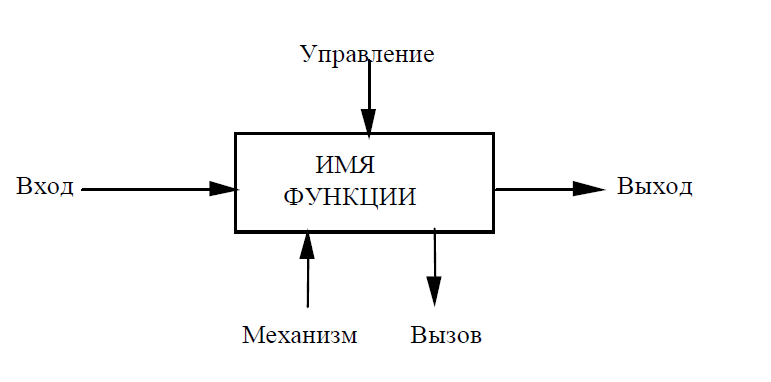
\includegraphics[width=0.4\linewidth]{semantics.png}
   \caption{Стандартное расположение стрелок}
   \label{img:semantics}
\end{figure}

\subsection{Диаграммы IDEF0}
IDEF0-модели состоят из трех типов документов: графических диаграмм, текста и глоссария. Эти документы имеют перекрестные ссылки друг на
друга. Графическая диаграмма – главный компонент IDEF0-модели, содержащий блоки, стрелки, соединения блоков и стрелок и ассоциированные с
ними отношения. Блоки представляют основные функции моделируемого объекта. Эти функции могут быть разбиты (декомпозированы) на составные
части и представлены в виде более подробных диаграмм; процесс декомпозиции продолжается до тех пор, пока объект не будет описан на уровне детализации, необходимом для достижения целей конкретного проекта. Диаграмма верхнего уровня обеспечивает наиболее общее или абстрактное описание объекта моделирования. За этой диаграммой следует серия дочерних диаграмм, дающих более детальное представление об объекте.

\subsection{Контекстная диаграмма верхнего уровня}
Каждая модель должна иметь контекстную диаграмму верхнего уровня, на которой объект моделирования представлен единственным блоком с граничными стрелками. Эта диаграмма называется A-0 (А минус нуль). Стрелки на этой диаграмме отображают связи объекта моделирования с окружающей средой. Поскольку единственный блок представляет весь объект, его имя -- общее для всего проекта. Это же справедливо и для всех стрелок диаграммы, поскольку они представляют полный комплект внешних интерфейсов объекта. Диаграмма A-0 устанавливает область моделирования и ее границу.

Контекстная диаграмма A-0 также должна содержать краткие утверждения, определяющие точку зрения должностного лица или подразделения, с позиций которого создается модель, и цель, для достижения которой ее разрабатывают. Эти утверждения помогают руководить разработкой модели и ввести этот процесс в определенные рамки. Точка зрения определяет, что и в каком разрезе можно увидеть в пределах контекста модели. Изменение точки зрения, приводит к рассмотрению других аспектов объекта. Аспекты, важные с одной точки зрения, могут не появиться в модели, разрабатываемой с другой точки зрения на тот же самый объект. Формулировка цели выражает причину создания модели, т.е. содержит перечень вопросов, на которые должна отвечать модель, что в значительной мере определяет ее структуру. Наиболее важные свойства объекта обычно выявляются на верхних уровнях иерархии; по мере декомпозиции функции верхнего уровня и разбиения ее на подфункции, эти свойства уточняются. Каждая подфункция, в свою очередь, декомпозируется на элементы следующего уровня, и так происходит до тех пор, пока не будет получена релевантная структура, позволяющая ответить на вопросы, сформулированные в цели моделирования. Каждая подфункция моделируется отдельным блоком Каждый родительский блок подробно описывается дочерней диаграммой на более низком уровне. Все дочерние диаграммы должны быть в пределах области контекстной диаграммы верхнего уровня.

\subsection{Дочерняя диаграмма}
Единственная функция, представленная на контекстной диаграмме верхнего уровня, может быть разложена на основные подфункции посредством создания дочерней диаграммы. В свою очередь, каждая из этих подфункций может быть разложена на составные части посредством создания дочерней диаграммы следующего, более низкого уровня, на которой некоторые или все функции также могут быть разложены на составные части. Каждая дочерняя диаграмма содержит дочерние блоки и стрелки, обеспечивающие дополнительную детализацию родительского блока. Дочерняя диаграмма, создаваемая при декомпозиции, охватывает ту же область, что и родительский блок, но описывает ее более подробно. Таким образом, дочерняя диаграмма как бы вложена в свой родительский блок. 

\subsection{Родительская диаграмма}
Родительская диаграмма --- та, которая содержит один или более родительских блоков. Каждая обычная (не-контекстная) диаграмма является также
дочерней диаграммой, поскольку, по определению, она подробно описывает некоторый родительский блок. Таким образом, любая диаграмма может быть как родительской диаграммой (содержать родительские блоки), так и дочерней (подробно описывать собственный родительский блок). Аналогично, блок может быть как родительским (подробно описываться дочерней диаграммой) так и дочерним (появляющимся на дочерней диаграмме). Основное иерархическое отношение существует между родительским блоком и дочерней диаграммой, которая его подробно описывает (рис.~\ref{img:struct}).

\begin{figure}[H]
   \centering
   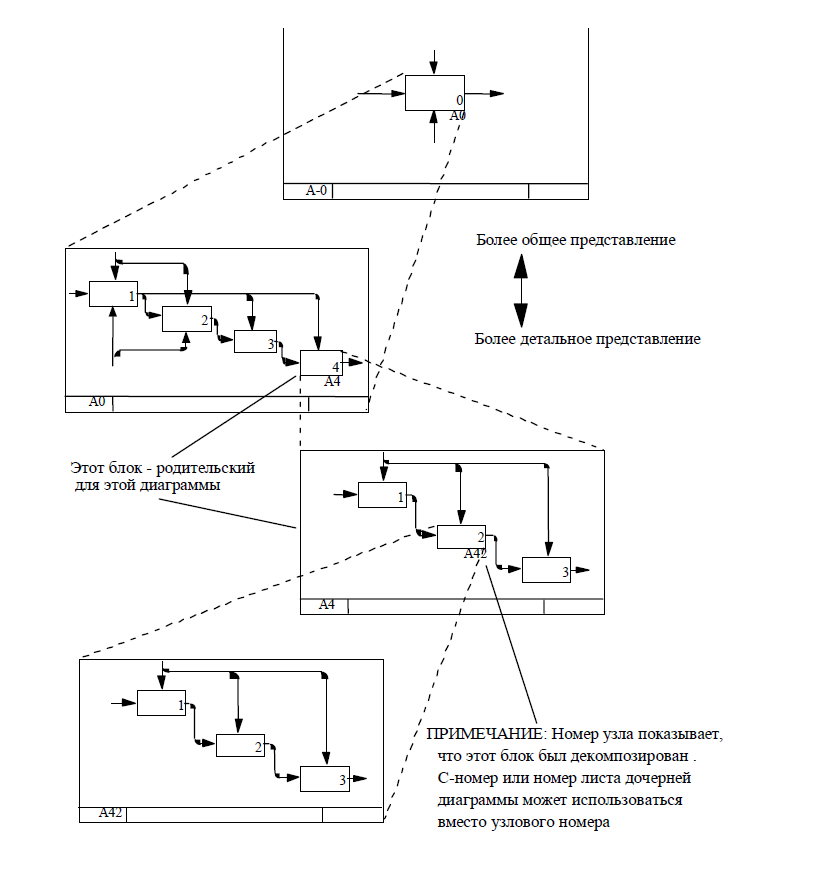
\includegraphics[width=0.5\linewidth]{struct.png}
   \caption{Иерархическое отношение между родительским блоком и дочерней диаграммой}
   \label{img:struct}
\end{figure}

\newpage
\section{Модель IDEF0 процесса разработки модуля кодирования и декодирования графа кодом Прюфера}
\subsection{Контекстная диаграмма А-0}

Моделирование процесса начинается именно с построения контекстной диаграммы. Эта диаграмма с единственным блоком определяет
контекст всей модели и образует основу для дальнейшей декомпозиции. 
\par На Рис. 5 педставлена диаграмма А-0. Контекстная диаграмма устанавливает область моделирования и границу 
области моделирования. Данная диаграмма задает основные параметры процесса разработки модуля кодирования и декодирования графа
кодом Прюфера с точки зрения разработчика-программиста. 

\par {\bf Входные данные:} техническое задание.

\par {\bf Выходные данные:} разработанный модуль кодирования и декодирования графа кодом Прюфера.

\par {\bf Управляющие данные:} нормативные документы.

\par {\bf Механизмы:} программист, язык программирования С++ и среда разработки Visual Studio 2022. 

\newpage
\hypertarget{img:A-0}{}
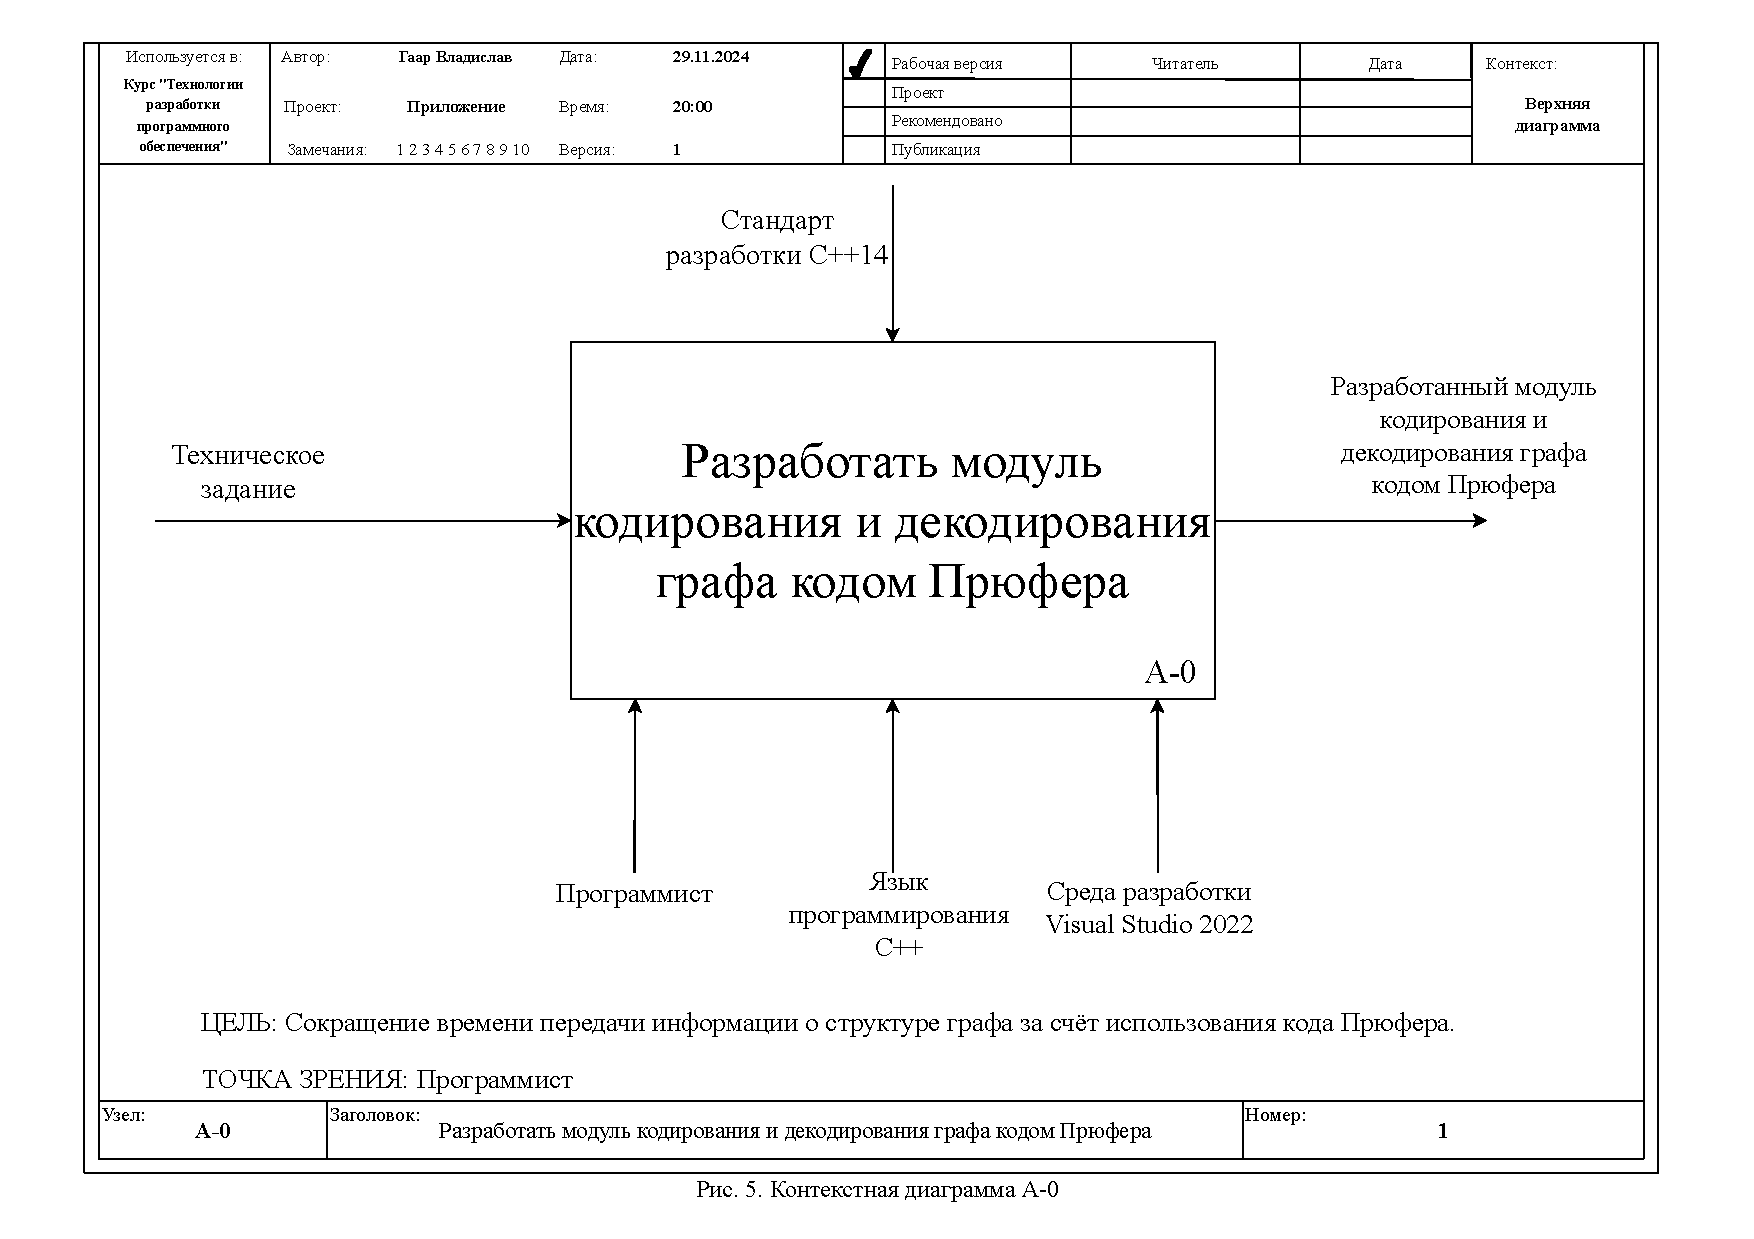
\includepdf[pages=1, fitpaper]{A-0.pdf}


\subsection{Диаграммы декомпозиций}
\subsubsection{Диаграмма А0}

На Рис. 6 представлена дочерняя диаграмма А0. Данная диаграмма представляет собой декомпозицию общего блока на 
элементы, которые связаны между собой.

Были выделены следующие блоки:

\begin{itemize}
	\item[A1.] Реализовать функции ввода данных и выбора способа задания графа;
	\item[A2.] Реализовать функцию генерации графа;
	\item[A3.] Реализовать функцию кодирования графа кодом Прюфера;
	\item[A4.] Реализовать функцию декодирования графа из кодов Прюфера;
	\item[A5.] Объединить реализованные функции.
\end{itemize} 

Управляющим воздействием всех блоков являются нормативные документы, механизмами являются язык программирования С++ 
и среда разработки Visual Studio 2022.

На вход блокам подается техническое задание на модуль кодирования и декодирования графа кодом Прюфера. На каждый 
блок поступают конкретные требования из технического задания, необходимые для разработки конкретных функций системы.

На выходе блоков получаются разработанные функции для работы с вводом данных, генерации графа, кодирования и декодирования графа кодом Прюфера.

Стрелки, входящие в блок и выходящие из него на диаграмме верхнего уровня, являются теми же самыми, что и стрелки, 
входящие в диаграмму нижнего уровня и выходящие из нее, потому что блок и диаграмма представляют одну и ту же 
часть системы. Как следствие этого, границы функции верхнего уровня -- это то же самое, что и границы диаграммы декомпозиции.

\newpage
\hypertarget{img:A0}{}
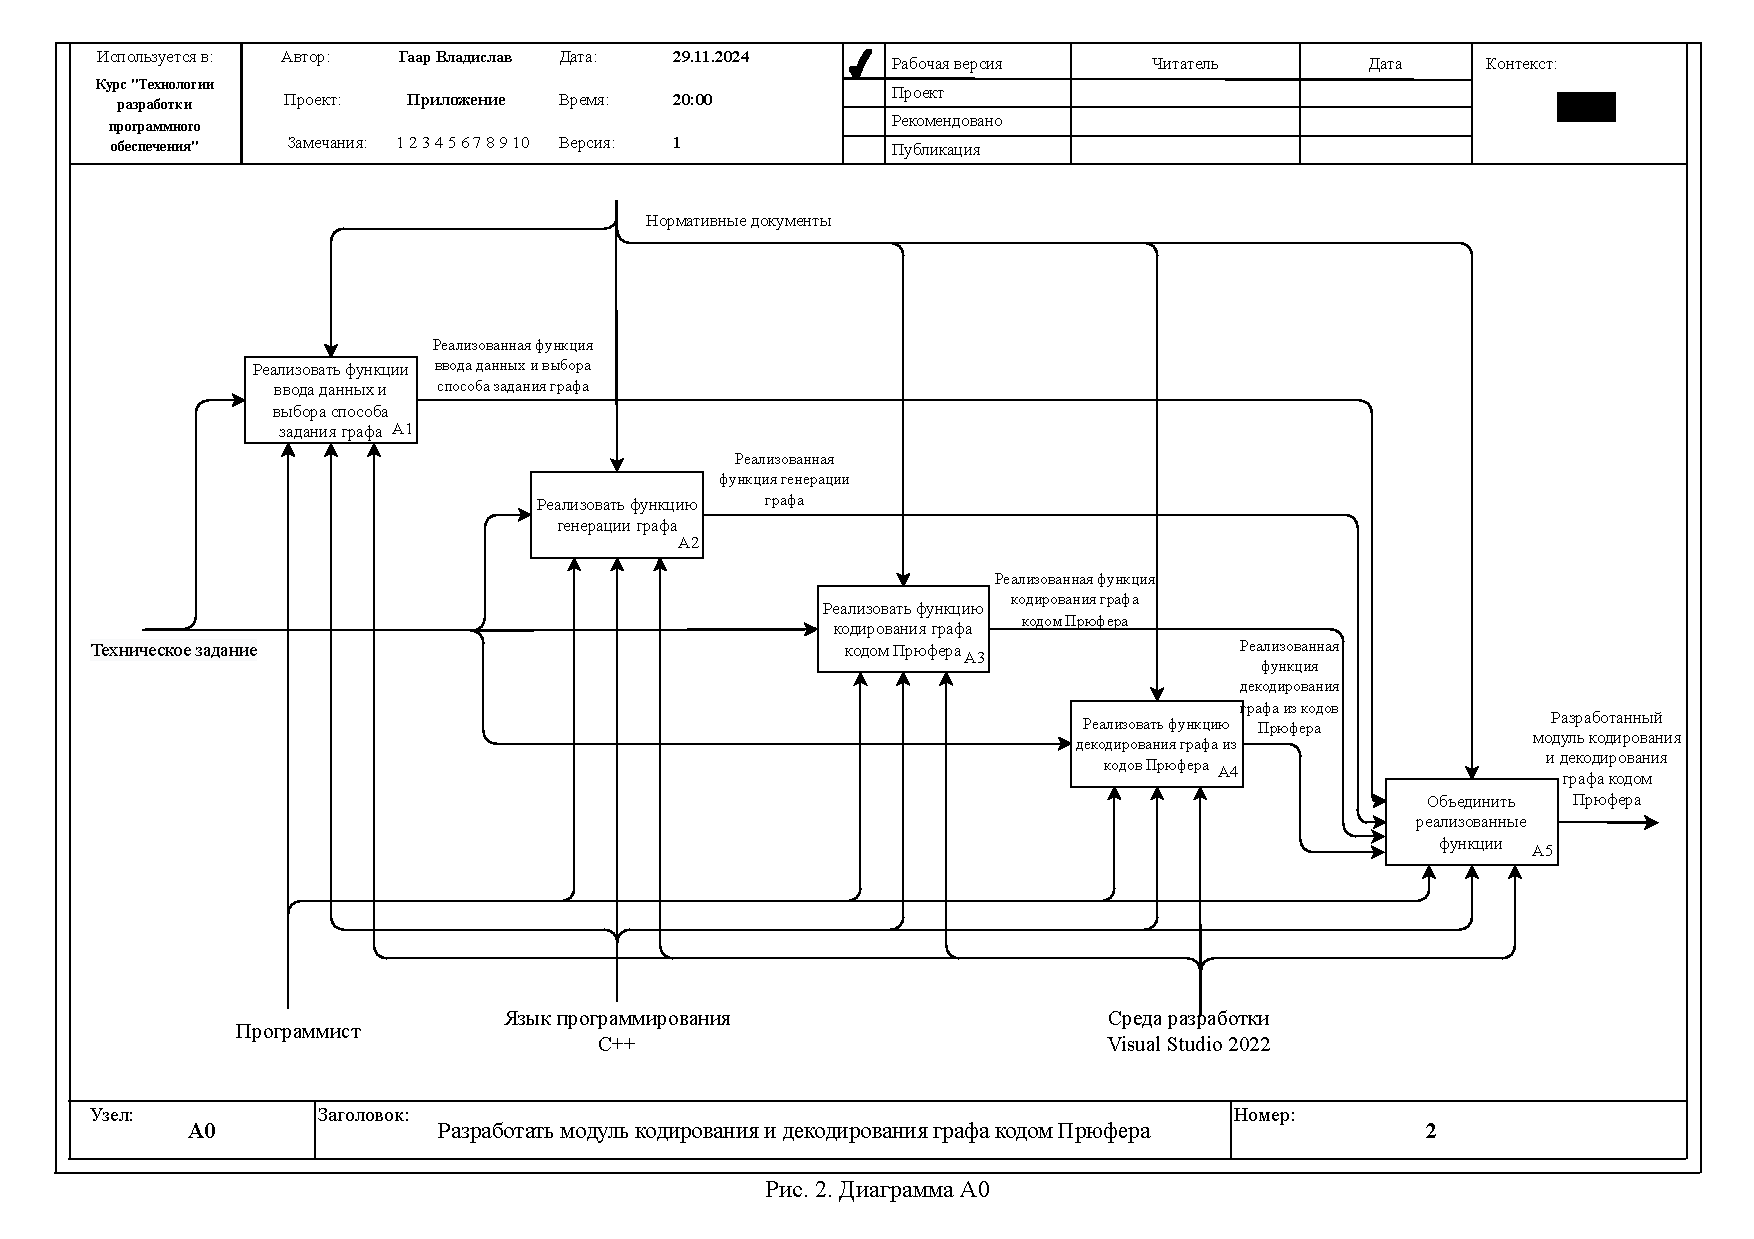
\includepdf[pages=1, fitpaper]{A0.pdf}


\subsubsection{Диаграмма А1}
Блок <<Реализовать функции ввода данных и выбора способа задания графа>> дочерней диаграммы А0 (см. Рис. 6) может быть разложен на составные части посредством создания дочерней диаграммы следующего, более низкого уровня.

На Рис. 7 представлена дочерняя диаграмма А1 более низкого уровня. Данная диаграмма представляет собой 
декомпозицию блока реализации функций ввода данных и выбора способа задания графа на элементы, которые связаны 
между собой. 

Были выделены следующие блоки:
\begin{itemize}
	\item[A11.] Релизовать функцию считывания количества вершин графа;
	\item[A12.] Реализовать функцию выбора способа задания графа;
	\item[A13.] Реализовать функцию подтверждения данных;
	\item[A14.] Объединить реализованные функции.
\end{itemize} 

На вход блокам поступают требования заказчика из ТЗ, относящиеся именно к функциям ввода данных и способу 
задания графа.

На выходе блоков получаются разработанные функции считывания количества вершин графа, выбора способа генерации графа,
подтверждения данных.

\newpage
\hypertarget{img:A1}{}
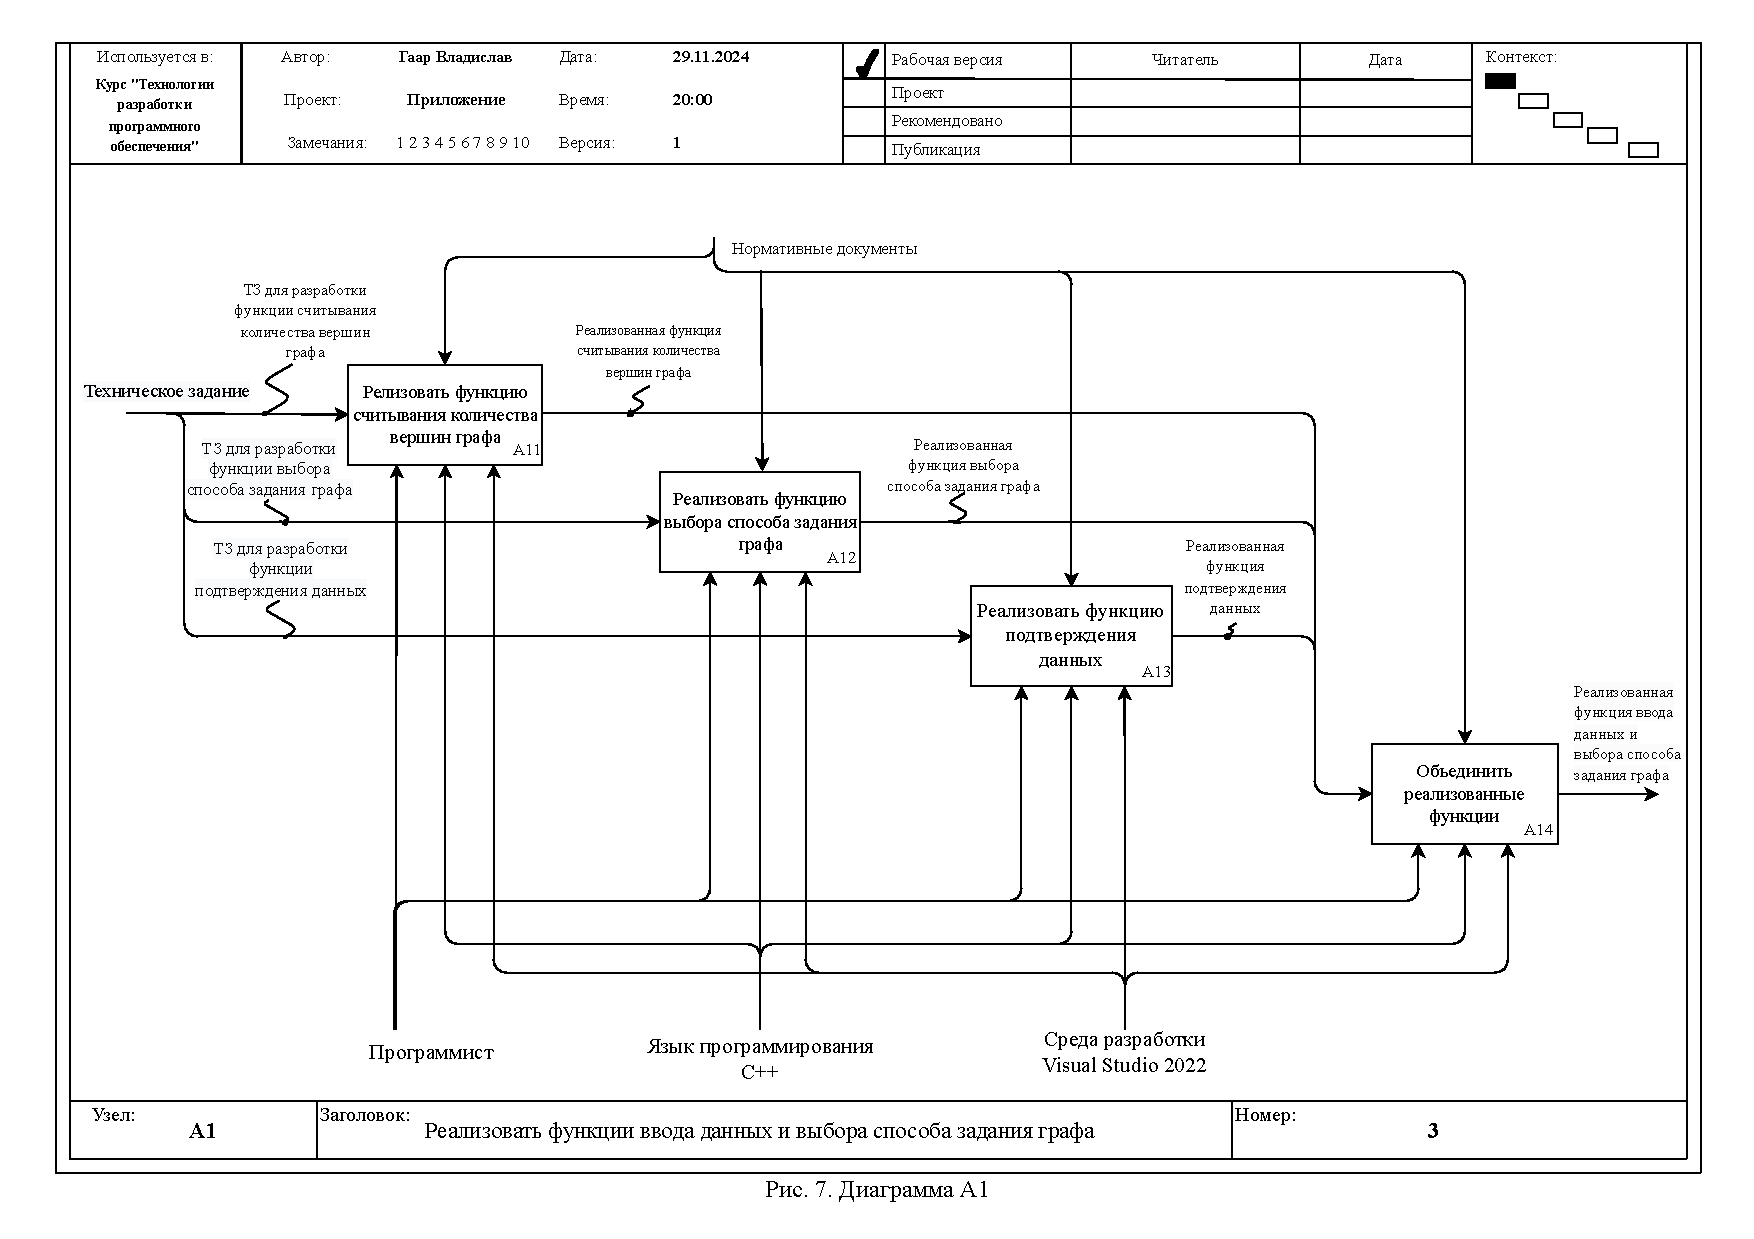
\includepdf[pages=1, fitpaper]{A1.pdf}


\subsubsection{Диаграмма А2}
На Рис. 8 представлено более подробное представление блока А2 <<Реализовать функцию генерации графа>>.

Диаграмма А2 является дочерней диаграммой для А0 (см. Рис. 6). Данная диаграмма представляет собой декомпозицию
блока реализации функции генерации графа на элементы, которые связаны между собой. 

Были выделены следующие блоки:
\begin{itemize}
	\item[A21.] Реализовать функцию генерации шаблона случайного графа
	\item[A22.] Релизовать функцию назначения весов рёбрам
	\item[A23.] Реализовать функцию проверки связности и ацикличности графа
	\item[A24.] Объединить реализованные функции
\end{itemize} 

\newpage
\hypertarget{img:A2}{}
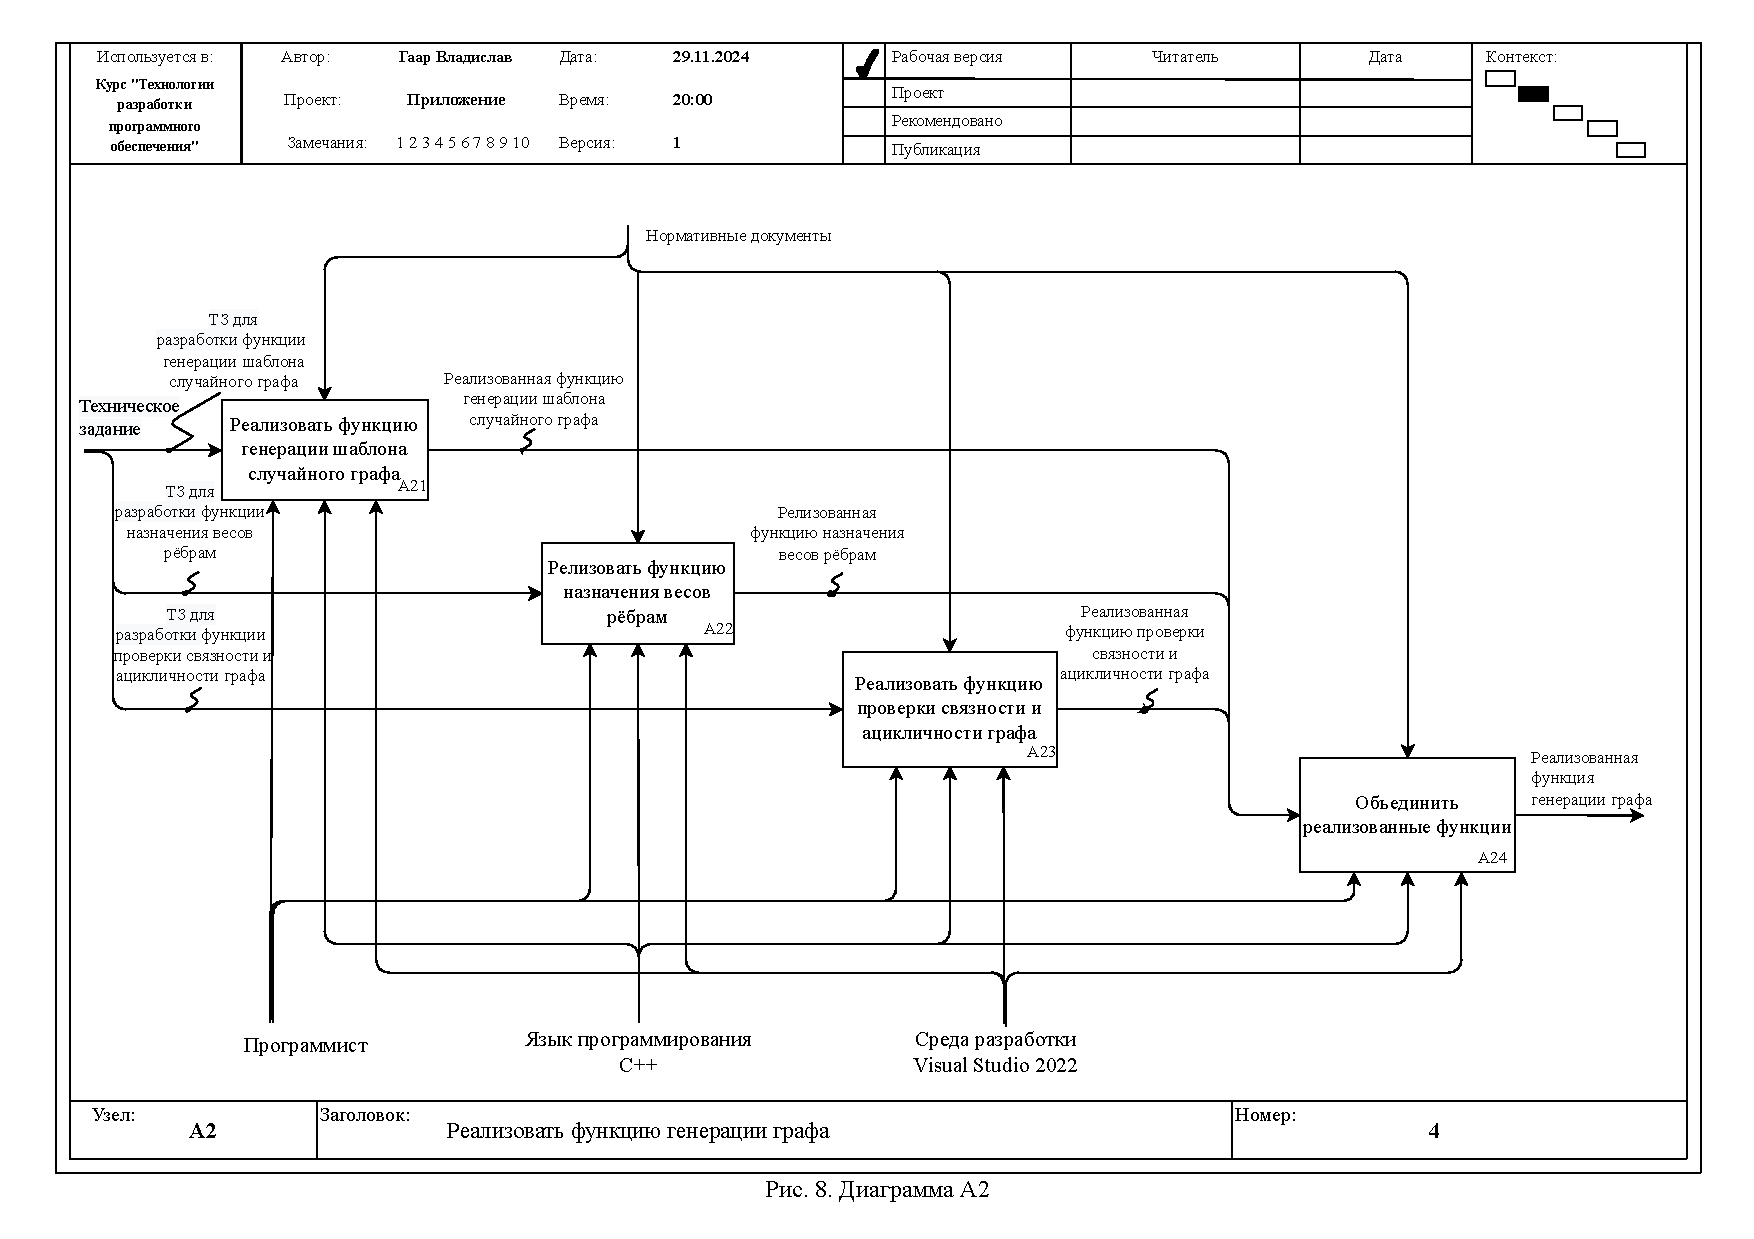
\includepdf[pages=1, fitpaper]{A2.pdf}


\cleardoublepage
\phantomsection
\newpage
\addcontentsline{toc}{section}{Заключение}
\section*{Заключение}
Таким образом, для разработки модели, демонстрирующей процесс создания модуля кодирования и декодирования графа кодом Прюфера,
была использована методология функционального моделирования IDEF0.

Благодаря данной методологии были выявлены и наглядно показаны основные этапы разработки приложения с точки зрения 
разработчика-программиста. Была построена контекстная диаграмма (родительская диаграмма), проведена ее декомпозиция и 
построены четыре дочерние диаграммы: А0, А1, А2. 

\cleardoublepage
\phantomsection
\newpage
%Список источников
\begin{thebibliography}{0}
	\bibitem{bib:gost_idef0}
	ГОССТАНДАРТ РОССИИ. Руководящий документ. МЕТОДОЛОГИЯ ФУНКЦИОНАЛЬНОГО МОДЕЛИРОВАНИЯ IDEF0. 
	Москва: ИПК Издательство стандартов, 2000г., 75с.

	\bibitem{bib:gost2_idef0}
	Методология IDEF0. Стандарт. Русская версия. МетаТехнология 1993, 91 с.

  \bibitem{bib:marka}
  Давид Марка, Клемент МакГоуэн, Методология структурного анализа и проектирования. Пер. с англ. М.:1993, 240 с., ISBN 5-7395-0007-9
\end{thebibliography}
\addcontentsline{toc}{section}{Список источников}

\end{document}